\chapter{Obecné}


\section{Model architektury}

Ať už použijeme DDA s online nebo offline adaptivitou, implicitní nebo explicitní, je zde spousta společných rysů, a proto je na místě vytvořit obecný model architektury dynamického vyvažování obtížnosti. Ve všech případech se snažíme podchytit zjednodušený model hráče na základě jeho projevů ve hře, a poté tyto informace dodáme hře, která herní svět upraví k lepšímu zážitku hráče.

Jeden z možných modelů DDA znázorňuje obr. \ref{fig:ch2ddaarch}. V principu se zaznamenávají akce hráče a herní proměnné jako je např. počet životů hráče. Na základě těchto logů se vytváří model hráče, model jeho zkušeností, dovedností, preferencí a osobnosti. Model hráče v kombinaci s aktuálním stavem hry slouží k odhadu očekávaného zážitku hráče v dalším stavu hry. A nakonec model zážitku s model výkonu hráče slouží jako vstup adaptačnímu a generačnímu enginu, který posléze upraví herní komponenty jakými je např. umělá inteligence NPC.

\begin{figure}
  \centering
  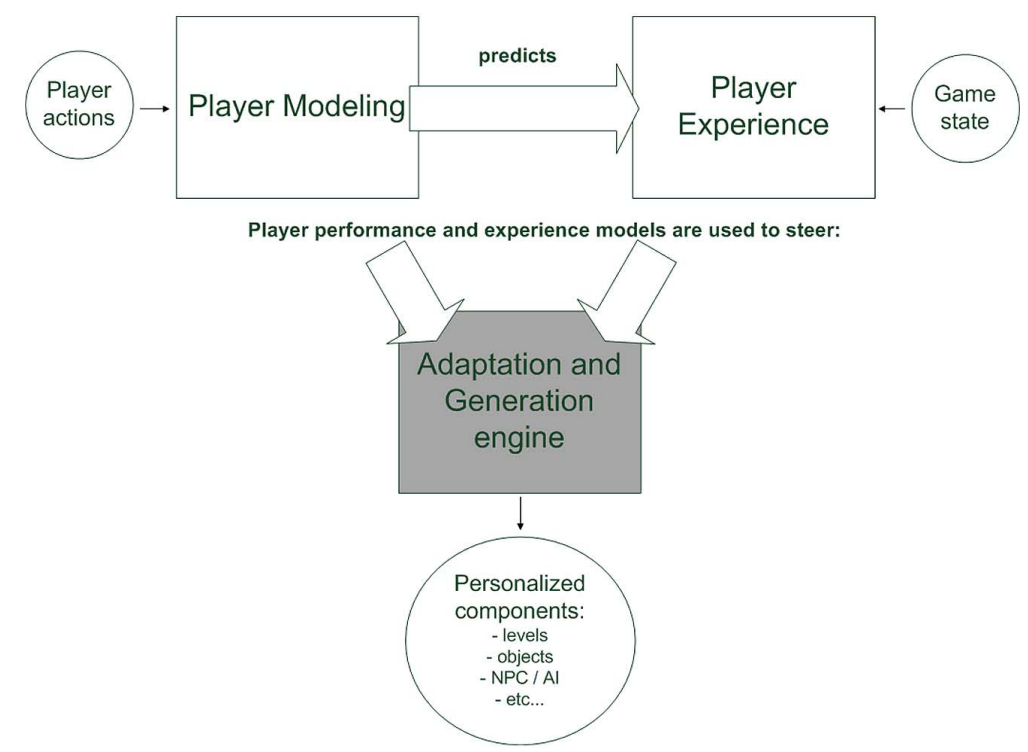
\includegraphics[width=0.75\textwidth]{ch2ddaarch}
	\caption{Přehled principů architektury adaptivních her. \cite{16Survey} }
	\label{fig:ch2ddaarch}
\end{figure}

V \cite{SwPatterns} se zabývali modelem DDA z pohledu návrhových vzorů objektového programování. Abstraktní model je znázorněn na obr. \ref{fig:ch2ddapatterns}. Senzory sbírají důležitá herní data, dle kterých se bude dále rozhodovat. Návrhový vzor Observer je připojen k Senzorům a v případě, že zaznamená zatelnou změnu v systému, vytvoří událost, trigger. Jednotlivé události jsou spojeny s akcemi a dohromady spolu tvoří pravidla uložená v databázi. V případě, že se spustí trigger spojený s akcí v některém z pravidel, rozhodne se v provedení této akce, což má na starost řadič, který má za úkol provést požadovanou změnu do stavu hry.

\begin{figure}
  \centering
  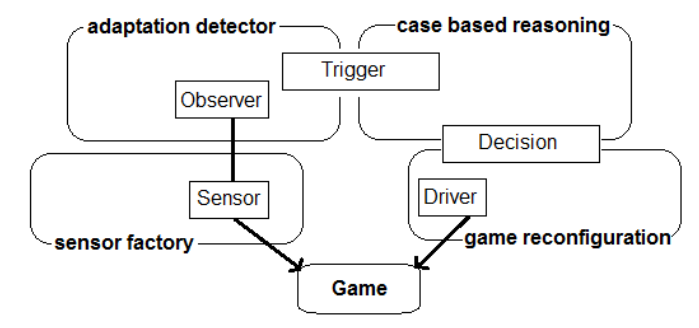
\includegraphics[width=0.75\textwidth]{ch2ddapatterns}
	\caption{Návrhové vzory DDA \cite{SwPatterns} }
	\label{fig:ch2ddapatterns}
\end{figure}

Dále se podíváme na jednotlivé návrhové vzory detailněji.

\subsection{Sensor factory}

Senzory jsou objekty, které pravidelně čtou herní data\footnote{Senzory nemusí zaznamenávat pouze herní data. Mohou zaznamenávat i prostředí uživatele např. pomocí Kinectu, nebo snímat aktuální tep hráče.} a upozorňují na změny zbytek DDA systému. Schéma návrhového vzoru znázorňuje obr. \ref{fig:ch2senzorfactory}. Senzor je abstraktní třídou, která zahrnuje periodické sbírání dat a upozorňující mechanismus. Konkrétní senzory z této třídy dědí a musí přepisovat abstraktní metodu refreshValue(), která zaznamenává konkrétní proměnnou systému. Třída SenzorFactory je zodpovědná za vytváření jednotlivých senzorů a je implementací návrhového vzoru factory. Továrna na senzory vyžaduje název senzoru a objekt, který má monitorovat. Vytvořené senzory si ukládá do registru. V případě, že uživatel zažádá o senzor, který už někdo vytvořil, dostane referenci na tento senzor. V opačném případě zkontroluje v ResourceManageru, jestli vytvořením nového senzoru se poruší některá z omezení zdrojů a pokud ne, senzor vytvoří.

\begin{figure}
  \centering
  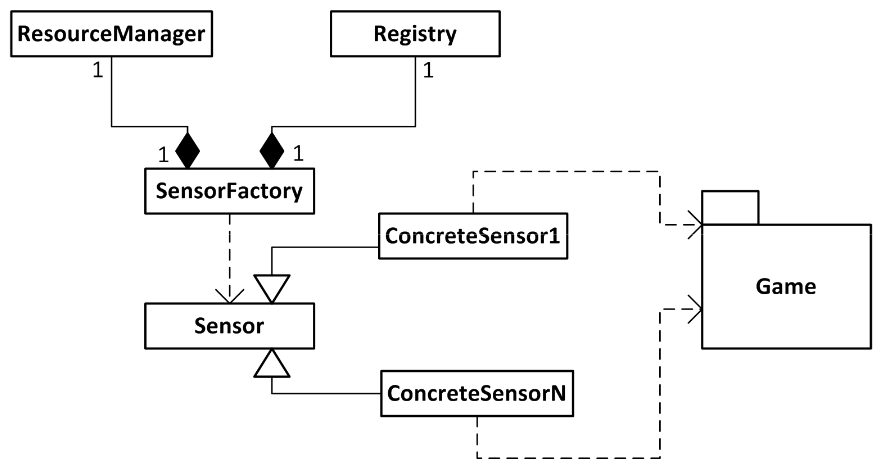
\includegraphics[width=0.5\textwidth]{ch2senzorfactory}
	\caption{Návrhový vzor sensor factory. \cite{SwPatterns} }
	\label{fig:ch2senzorfactory}
\end{figure}

\subsection{Adaptation detector}

Hrubá data získaná senzory se musí dále zpracovat. Tyto data získává AdaptationDetector pomocí observeru z návrhového vzoru senzor-observer. Na tomto místě se rozhoduje, jestli senzory již zaznamenaly dostatečnou změnu systému. Nedostatečnou změnou může být vystřelení jednoho náboje z plně nabitého revolveru. Naopak vystřílení půlky zásobníku může být významné. O významnost změny se stará TreshholdAnalyzer s Tresholdem. Treshold uchovává parametr hranice a její typ. (menší rovno, větší apod.) V případě dosažení prahu TresholdAnalyzer dá vědět AdaptationDetectoru, který vytvoří trigger, spouštěč. Trigger s sebou může nést další dodatečné informace jako je např. množství přeživších nepřátel. Viz obr. \ref{fig:ch2adaptationdesing}.

\begin{figure}
  \centering
  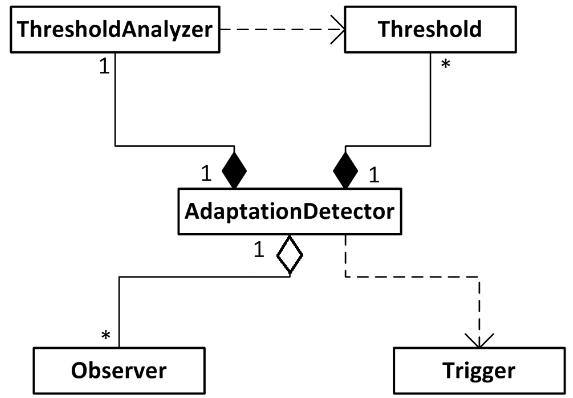
\includegraphics[width=0.5\textwidth]{ch2adaptationdesing}
	\caption{Návrhový vzor sensor factory. \cite{SwPatterns} }
	\label{fig:ch2adaptationdesing}
\end{figure}

\subsection{Case based reasoning}

Trigger spustí rozhodování na základě případů. Tento návrhový vzor(obr. \ref{fig:ch2casebase}) se použije, jestliže je možné vyvažování obtížnosti definovat konečným množstvím případů. InferenceEngine obsahuje dvě datové struktury: TriggerPool a FixedRules. Fixed rules obsahují pravidla, která jsou úzce spojená s konkrétní hrou. Pravidlo je kombinací triggeru a akce/rozhodnutí. TriggerPool funguje jako fronta událostí. Do fronty se řadí spuštěné triggery a jsou obsluhovány od nejstaršího. InferenceEngine vždy odebere jeden trigger z poolu, najde ho v databázi FixedRules pravidel a s ním nalezne vhodné rozhodnutí, které se má dále provést.

\begin{figure}
  \centering
  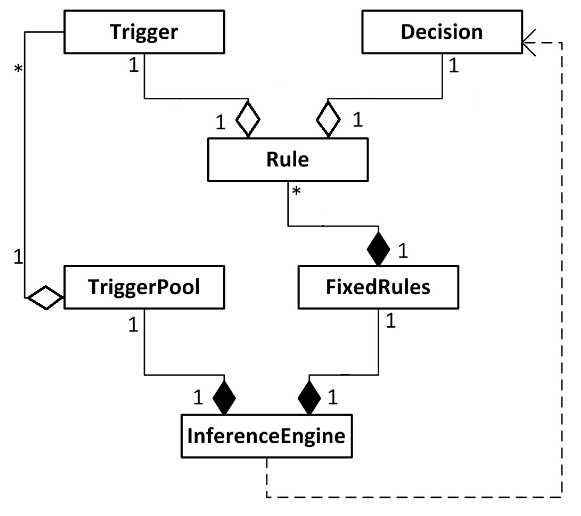
\includegraphics[width=0.5\textwidth]{ch2casebase}
	\caption{Návrhový vzor Case based reasoning. \cite{SwPatterns} }
	\label{fig:ch2casebase}
\end{figure}

\subsection{Game reconfiguration}

Posledním krokem je provedení požadované změny v herním světě. Návrhový vzor Game reconfiguration(obr. \ref{fig:ch2gamereco}) v sobě obsahuje jiný návrhový vzor, adapter. AdaptationDriver dostane ke zpracování rozhodnutí z InferenceEnginu. AdaptationDriver provede rozhodnutí za pomoci Driveru. Driver mění objekty, jež implementují rozhraní State, přes které zjišťuje aktuální stav objektu. S provedením jeho změny čeká dokud se nestane objekt neaktivním.

\begin{figure}
  \centering
  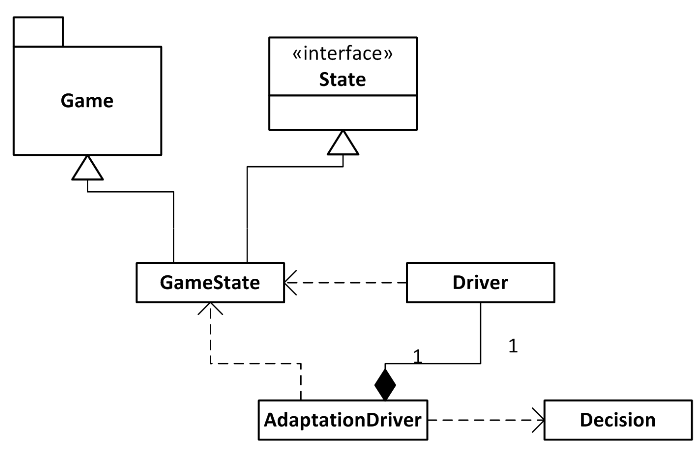
\includegraphics[width=0.5\textwidth]{ch2gamereco}
	\caption{Návrhový vzor Game reconfiguration. \cite{SwPatterns} }
	\label{fig:ch2gamereco}
\end{figure}

\section{Definice zábavnosti}  \label{sec:defzab}

\section{Flow}

\section{Metriky}

